\chapter{Algorithmen und Methoden}

\begin{table}[h]
    \centering
    \begin{tabularx}{\textwidth}{|X|X|X|X|X|}
        \hline
        Router & Raum 1      & Raum 2      & Raum 3     & Unbekannt (1) \\ \hline
        1      & -73.67 dBm  & -91.12 dBm  & -69.37 dBm & -73.51 dBm    \\ \hline
        2      & -104.99 dBm & -64.47 dBm  & -89.65 dBm & -103.41 dBm   \\ \hline
        3      & -67.03 dBm  & -105.38 dBm & -88.40 dBm & -70.35 dBm    \\ \hline
    \end{tabularx}
    \caption{RSSI-Werte für die drei Router und die Räume}
    \label{tab:rssi_values}
\end{table}

\paragraph{Quellen für Auswahl}

\begin{itemize}
    \item https://ar5iv.labs.arxiv.org/html/2111.14281 -> KNN, SVM
    \item A Wireless Fingerprint Location Method Based on Target Tracking (Kapitel 3, Seite 3) -> KNN, SVM, Random Forest
    \item https://onlinelibrary.wiley.com/doi/full/10.1155/2017/6268797 -> KNN, SVM, Random Forest. In Table 2 stehen die Genauigkeiten der Algorithmen
\end{itemize}

\section{K-Nearest Neighbors (KNN)}
\textbf{Quellen:} \\
\href{https://www.ibm.com/de-de/topics/knn}{Quelle 1: https://www.ibm.com/de-de/topics/knn} \\
Quelle 4: Comprehensive analysis of distance and similarity measures for Wi-Fi fingerprinting indoor positioning systems \\
Quelle 5: Hechenbichler, Schliep: - Weighted k-Nearest-Neighbor Techniques and Ordinal Classification

\subsection{Algorithmusbeschreibung}
\textbf{Quelle 1:} Der k-nearest neighbor (KNN) Algorithmus ist ein überwachter Lernklassifikator, der auf dem Konzept der Nähe basiert und zur Lösung von Klassifikations- und Regressionsproblemen verwendet werden kann. Der Algorithmus funktioniert so, dass ein Datenpunkt mit den vorhandenen Datenpunkten in den Trainingsdaten verglichen wird und die Distanz zu jedem Datenpunkt berechnet wird. Basierend auf diesen Distanzen werden die k Datenpunkte ausgewählt, die den kleinsten Abstand haben. Aus diesen k Datenpunkten wird dann die Klasse bestimmt, die am häufigsten vertreten ist. Hierbei reicht bereits eine relative Mehrheit aus (wenn z.B. 4 Klassen vertreten sind, kann ein Anteil von mehr als 25 \% ausreichend sein).

\subsection{Distanzmetriken (euklidisch, Sorensen)}
\textbf{Quelle 1:} Für die Berechnung der Distanzen können verschiedene Distanzmetriken verwendet werden. Die am häufigsten verwendete Distanzmetrik ist der euklidische Abstand. In dieser Arbeit wurde entschieden, sowohl die euklidische Distanz als auch die Sorensen-Distanz zu verwenden. Bei der euklidischen Distanz wird das Quadrat der Abstände (Betrag der Differenz) zwischen zwei Werten gebildet, über alle Wertepaare aufsummiert und abschließend die Quadratwurzel dieser Summe gezogen (siehe \ref{eq:euclidean}).

\begin{equation}
    \label{eq:euclidean}
    \text{distance}_{\text{euclidean}}(P, Q) = \sqrt{\sum_{i=1}^{d} (P_i - Q_i)^2}
\end{equation}

\textbf{Quelle 4:} Bei der Sorensen-Distanzfunktion werden die Abstände der Datenpunkte aufsummiert und durch die Summe der Wertepaare zweier Datenpunkte geteilt (siehe \ref{eq:sorensen}). Grund für die Wahl dieser beiden Metriken: Die Arbeit "Comprehensive analysis of distance and similarity measures for Wi-Fi fingerprinting indoor positioning systems" konnte damit gute Ergebnisse erzielen. Der euklidische Abstand ist weit verbreitet und entspricht auch der bisherigen Implementierung in der App.

\begin{equation}
    \label{eq:sorensen}
    \text{distance}_{\text{sorensen}}(P, Q) = \frac{\sum_{i=1}^{d} |P_i - Q_i|}{\sum_{i=1}^{d} (P_i + Q_i)}
\end{equation}

In Abbildung \ref{fig:distance_metrics_heatmaps} sind die Heatmaps für die beiden Distanzmetriken dargestellt.

Damit die Unterschiede zwischen den beiden Distanzmetriken besser sichtbar sind, wurden die Distanzen zwischen allen möglichen Wertepaaren zwischen 0 und -100 berechnet und in Abbildung \ref{fig:distance_metrics_heatmaps} dargestellt. Wie zu erkennen ist, sind diese beiden symmetrisch zu der Geraden zwischen den beiden Punkten (0, 0) und (-100, -100). Wie zu erkennen ist, sind die Werte für die euklidische Distanz auch symmetrisch zu der Geraden zwischen den beiden Punkten (0, -100) und (-100, 0). Dementsprechend ist die Distanz alleine von der Differenz der beiden Werte abhängig. Bei der Sørensen-Distanz muss bei kleineren Werten der Abstand größer sein, um die gleiche Distanz zu erreichen wie bei kleineren Werten.

Um dies zu verdeutlichen, betrachten wir die Berechnung der Distanzen für zwei Beispielwertepaare:

Gegeben:
\begin{itemize}
    \item Wertepaar 1: \( P = -30 \, \text{dBm} \), \( Q = -40 \, \text{dBm} \)
    \item Wertepaar 2: \( P = -70 \, \text{dBm} \), \( Q = -80 \, \text{dBm} \)
\end{itemize}

\begin{table}[H]
    \centering
    \begin{tabular}{|c|c|c|}
        \hline
        Wertepaar                                & Sørensen-Dice Distanz & Euklidische Distanz \\
        \hline
        \(-30 \, \text{dBm}, -40 \, \text{dBm}\) & \(-0.142857\)         & \(10\)              \\
        \(-70 \, \text{dBm}, -80 \, \text{dBm}\) & \(-0.066667\)         & \(10\)              \\
        \hline
    \end{tabular}
    \caption{Berechnete Distanzen für die gegebenen Wertepaare}
    \label{tab:distance_results}
\end{table}

\begin{figure}[H]
    \centering
    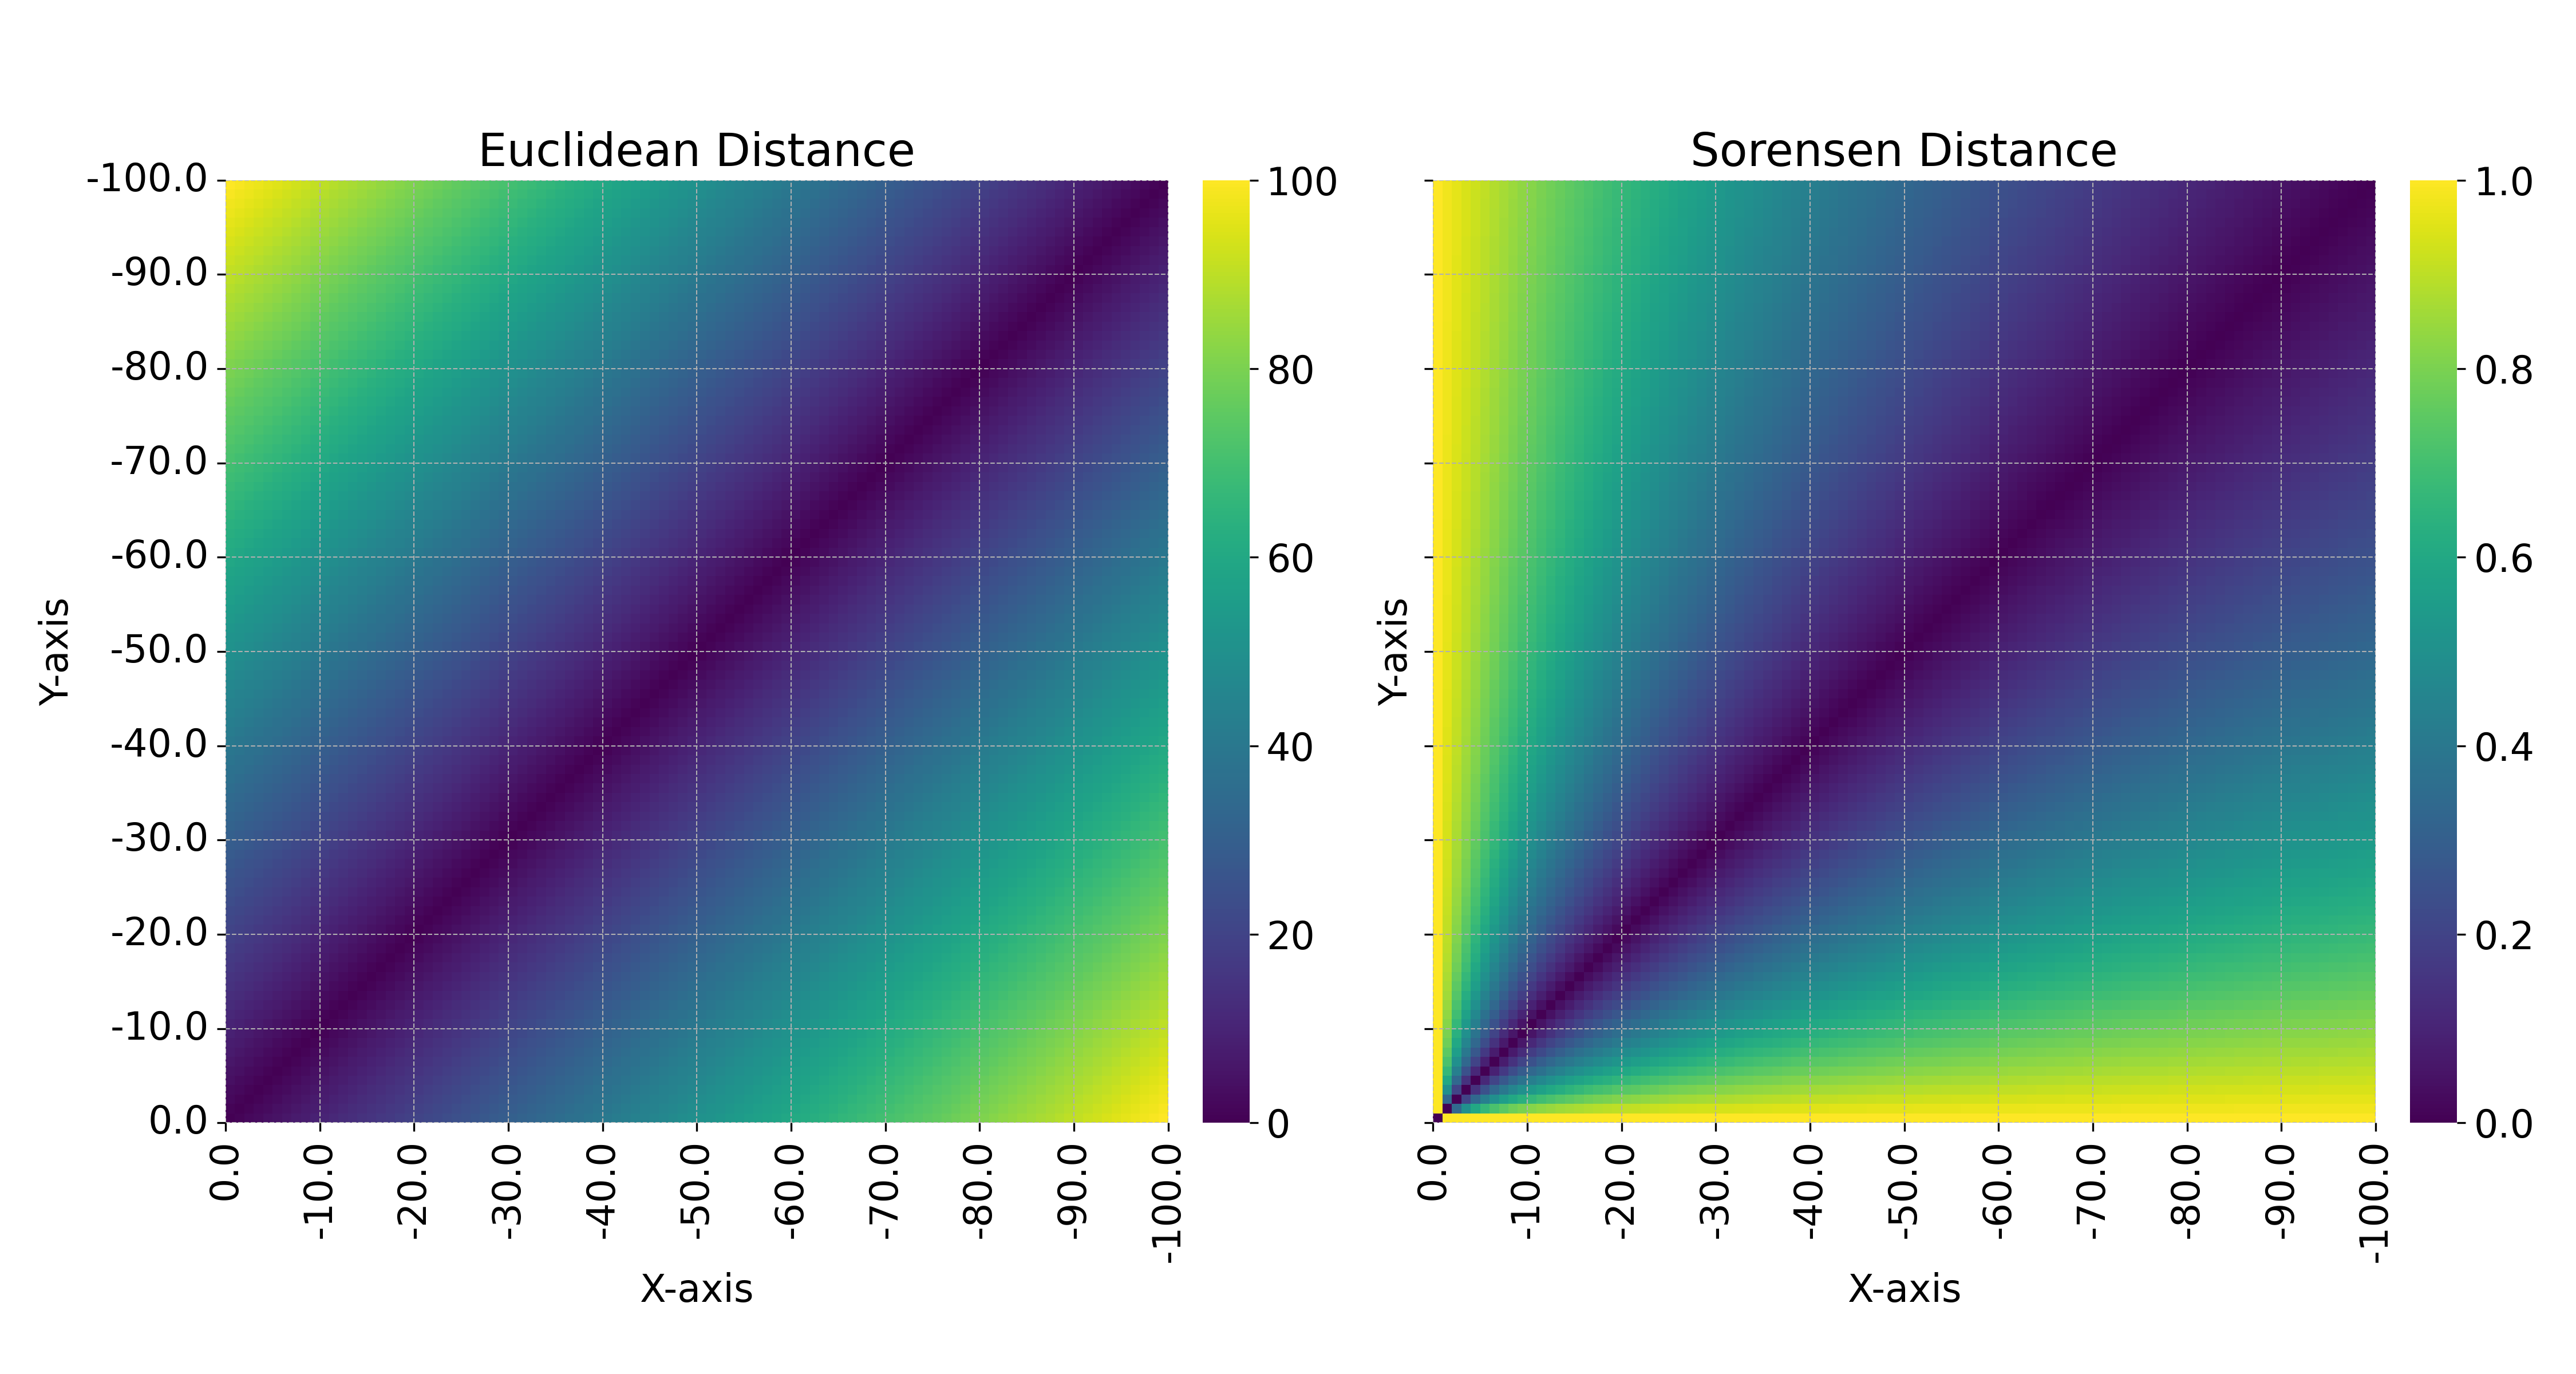
\includegraphics[width=0.8\textwidth]{images/distance_metrics_heatmaps.png}
    \caption{Euclidean vs. Sorensen distance metrics}
    \label{fig:distance_metrics_heatmaps}
\end{figure}



\subsection{Gewichtung (uniform vs. distance)}
\textbf{Quelle 5:}
\begin{itemize}
    \item Die Erweiterung basiert auf der Idee, dass Beobachtungen im Trainingsset, die besonders nahe an der neuen Beobachtung (y, x) liegen, ein höheres Gewicht in der Entscheidungsfindung erhalten sollten als weiter entfernte Nachbarn.
    \item Im klassischen kNN beeinflussen nur die k nächsten Nachbarn die Vorhersage.
    \item Der Einfluss jedes der k nächsten Nachbarn ist gleich, obwohl die individuelle Ähnlichkeit zu (y, x) stark variieren kann.
    \item Um dieses Ziel zu erreichen, müssen die Distanzen, die bei der Suche nach den nächsten Nachbarn im ersten Schritt verwendet werden, in Ähnlichkeitsmaße umgewandelt werden, die als Gewichte verwendet werden können.
\end{itemize}

\subsection{Parameter: Anzahl der Nachbarn}
\textbf{Quelle 1:} Der Parameter k legt fest, wie viele nächste Nachbarn für die Klassifizierung ausgewählt werden. Für k = 1 wird nur der nächste Nachbar ausgewählt, wodurch kein Mehrheitsvotum stattfindet. Bei kleinen Werten für k kann eine hohe Varianz und eine geringe Verzerrung auftreten, während bei größeren Werten die Varianz geringer und die Verzerrung höher ist. Die Auswahl von k hängt stark von den vorhandenen Trainingsdaten ab. Bei Daten mit Ausreißern und Rauschen wird empfohlen, höhere Werte für k zu wählen, da in diesen Fällen bessere Ergebnisse erzielt werden. Zudem wird empfohlen, ungerade Werte für k zu wählen, um Unentschieden beim Mehrheitsvotum zu vermeiden.

\section{Support Vector Machines (SVM)}


In Abbildung \ref{fig:myplot_7_svm} ist ein SVM dargestellt.

\begin{figure}[H]
    \centering
    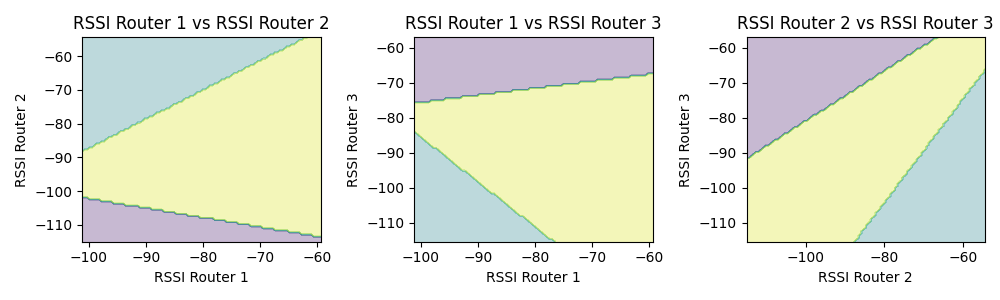
\includegraphics[width=0.8\textwidth]{images/myplot_7_svm.png}
    \caption{SVM}
    \label{fig:myplot_7_svm}
\end{figure}

\textbf{Quellen:} \\
\href{https://www.bigdata-insider.de/was-ist-eine-support-vector-machine-a-880134}{Quelle 6: https://www.bigdata-insider.de/was-ist-eine-support-vector-machine-a-880134} \\
\href{https://www.ibm.com/topics/support-vector-machine}{Quelle 7: https://www.ibm.com/topics/support-vector-machine} \\
\href{https://wires.onlinelibrary.wiley.com/doi/full/10.1002/wics.49}{Quelle 8: https://wires.onlinelibrary.wiley.com/doi/full/10.1002/wics.49}


Quelle warum gerade RBF: An Indoor Localization of WiFi Based on Support Vector Machines

\subsection{Algorithmusbeschreibung}
\textbf{Quelle 7:} Der Support Vector Machine (SVM) Algorithmus ist ein überwachter maschineller Lernalgorithmus, der verwendet wird, um Daten zu klassifizieren. Die Klassifizierung erfolgt, indem die optimale Trennlinie – die sogenannte Hyperebene – zwischen den Datenpunkten gefunden wird. Diese Hyperebene wird so positioniert, dass der maximale Abstand zwischen den Datenpunkten der beiden Klassen erreicht wird. SVM kann sowohl mit linear trennbaren Daten als auch mit nicht linear trennbaren Daten arbeiten. Bei nicht linearen Daten wird der sogenannte Kernel-Trick angewendet, bei dem die Daten mithilfe einer Kernel-Funktion in einen höherdimensionalen Raum transformiert werden.

\subsection{Kernel (linear, RBF)}
\textbf{Quelle 7:} Bei der linearen Klassifizierung werden die Datenpunkte durch eine Linie oder Ebene getrennt und nicht transformiert. Bei nicht linearen SVMs wird zuerst die Kernel-Methode angewendet, und anschließend werden die Daten linear getrennt. In dieser Arbeit wurde entschieden, ein lineares und ein nicht lineares SVM zu vergleichen. Für das nicht lineare SVM wurde der RBF-Kernel gewählt, da in der Arbeit "Device-Free Presence Detection and Localization With SVM and CSI Fingerprinting" mit diesem Kernel die besten Ergebnisse unter den nicht linearen SVMs erzielt wurden.

\subsection{Parameter: Regularisierungsparameter C und Kernel-Parameter gamma}
\textbf{Quelle 7:} Mit dem Parameter C kann der Margin angepasst werden. Ein größerer Wert verengt den Margin für eine minimale Fehlklassifizierung und ein größerer Wert für C erweitert den Margin, sodass mehr Fehlklassifizierungen zugelassen werden. Gamma kontrolliert den Einfluss eines einzelnen Datenpunktes. Ein höherer Wert sorgt für eine kleinere Einflussreichweite, wodurch die Entscheidungsgrenzen enger werden. Der Parameter Gamma kann nur bei nicht linearen SVMs verwendet werden. \\
Quelle für die Auswahl der Parameter Werte: Semi-Supervised Classification by Low Density Separation

\section{Random Forest}

Gute quelle: WiFi Indoor Localization with CSI Fingerprinting-Based Random Forest -> Wie wichtig ist welcher Hyperparameter?

In Abbildung \ref{fig:myplot_7_rf} ist ein Entscheidungsbaum dargestellt.

\begin{figure}[H]
    \centering
    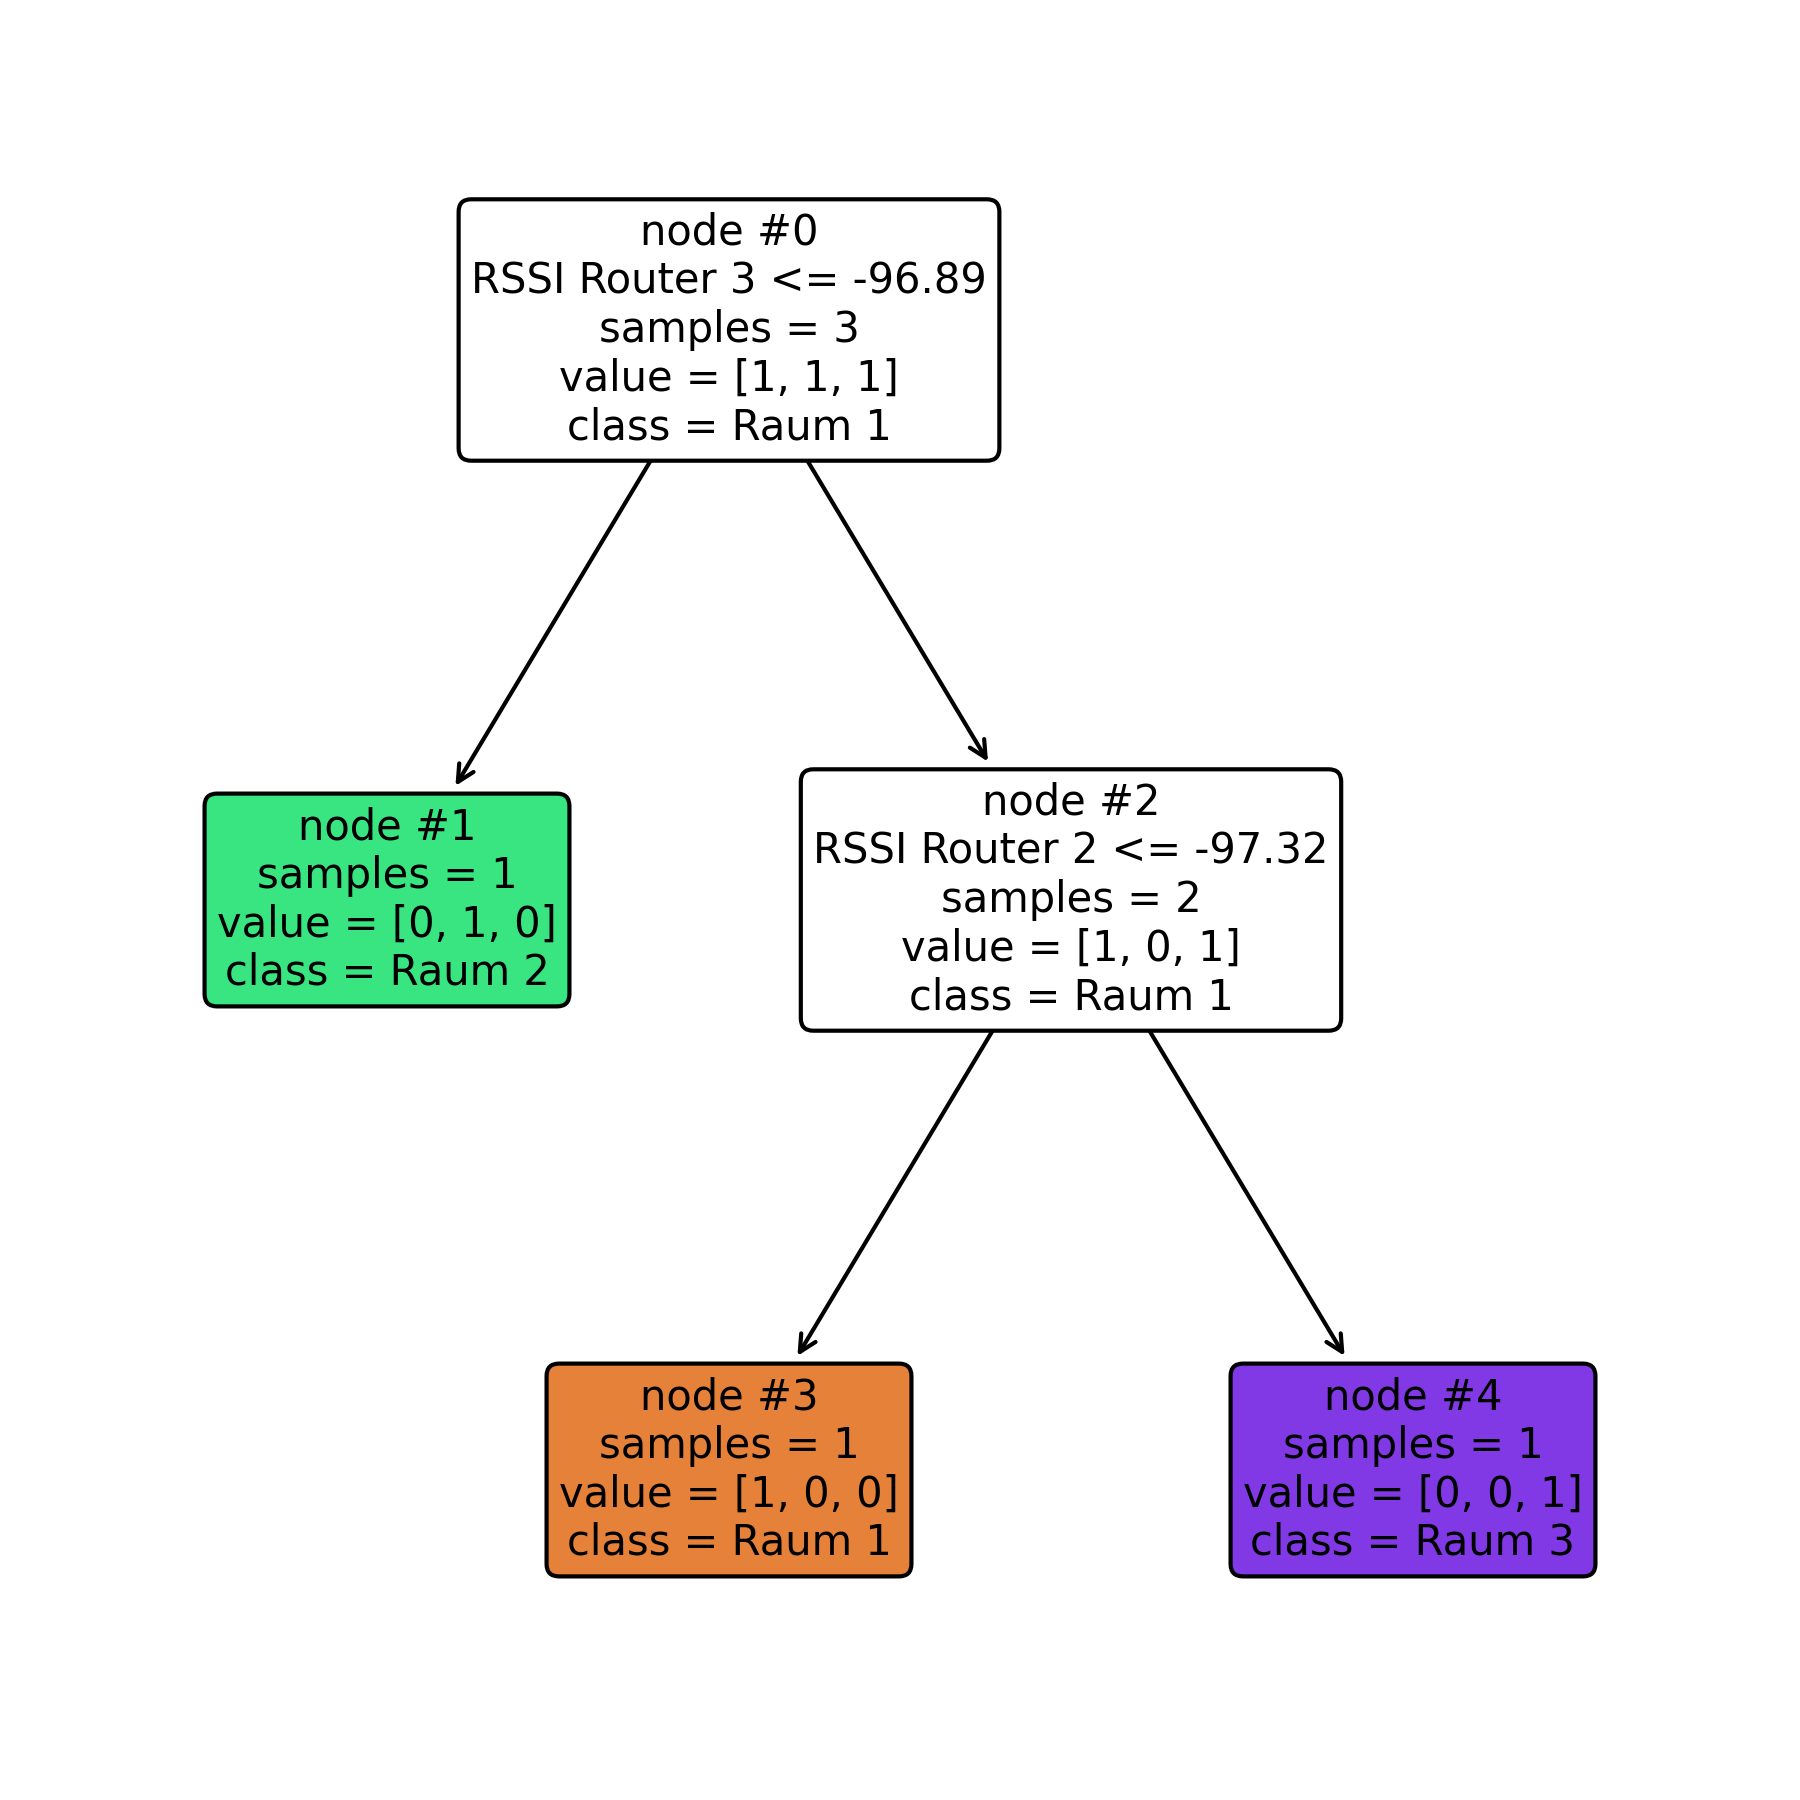
\includegraphics[width=0.8\textwidth]{images/myplot_7_rf.png}
    \caption{Distance vs. Uniform weights}
    \label{fig:myplot_7_rf}
\end{figure}

\textbf{Quelle:} \\
\href{https://builtin.com/data-science/random-forest-algorithm}{Quelle 9: https://builtin.com/data-science/random-forest-algorithm}

\subsection{Algorithmusbeschreibung}
\textbf{Quelle 9:} Der Random Forest Algorithmus ist ein überwachter Lernalgorithmus, der eine Menge an Entscheidungsbäumen erstellt. Ein Entscheidungsbaum besteht aus Knoten, welche eine Bedingung zu einem der Merkmale aus dem Datenset abfragen. Zum Beispiel sowas wie: Ist der RSSI-Wert von Access Point 1 größer gleich -80 dBm? Je nachdem wie diese Frage beantwortet wird, geht es dann zum nächsten Knoten usw. Am Ende jedes Strangs

\subsection{Parameter: Anzahl der Bäume (n\_estimators)}
